\documentclass[a4paper, 11pt]{article}
\usepackage[utf8]{inputenc} % Change according your file encoding
\usepackage[margin=1in]{geometry}
\usepackage{graphicx}
\usepackage{caption}
\usepackage{subcaption}
\usepackage{float}
\usepackage[catalan,english]{babel}


%% Estil de Paràgraf
\setlength{\parskip}{4mm}
\setlength{\parindent}{0mm}

%% Estil lletra
\renewcommand{\familydefault}{\sfdefault}

\title{Activitat 7 - Web 2.0/25M}
\author{Ismael Peral Álvarez, Ferran Arau Castell}
\date{\today}

\begin{document}

\maketitle

\section{Introducció}

El projecte consisteix en dissenyar i arquitecturar la infraestructura necesària per allotjar una aplicació web. Concretament es tracta d'una aplicació intensiva en imatges que ha de servir a centenars d'usuaris i ha de estar disponible 24 hores al dia, 7 dies a la setmana.

El pressupost disponible és de 25 millons d'euros, amb els quals caldrà assumir els costos Capex i Opex. En conseqüència, cal provisionar els servidors de l'aplicació, els equips de xarxa i les cabines de discs. Cal assumir el cost dels serveis de housing, backup, xarxa i electricitat. Possiblement al llarg del projecte es modifiquin alguns d'aquests punts, segons les decisions que es prenguin.

La aplicació web amb la que es treballarà requerirà un model de tràfic vertical entre la plataforma i internet. Principalment amb un ample de banda de pujada de dades molt significatiu. És per aquest motiu, que sembla que caldrà fer un esforç econòmic important en les prestacions de la xarxa.


\section{Requisits}

Els requisits mostren que cal disposar d'una infraestructura en alta disponibilitat i amb capacitat de creixement, és a dir, una infraestructura escalable horitzontalment. També s'estableix una SLA; cal garantir un temps de resposta inferior o igual a 100ms per petició HTTP. El qual significa, que cal servir un mínim de 10 peticions per segon.

Per poder complir els requisits cal desenvolupar una sèrie d'assumpcions, les quals es tractarà que siguin el més realistes possible. En primer lloc, cada petició tindrà un tamany mig de 600 bytes i cada resposta serà en mitjana de 180 KBytes. Cada petició generarà 5 accessos a disc d'un KByte cadascuna.

En quan a l'arquitectura, s'assumirà que l'aplicació no tindrà una capa de Base de Dades. No obstant, sí disposarà d'una capa d'aplicació on s'executarà el codi dinàmic d'aquesta. En l'apartat d'especificació de l'arquitectura es definirà una capa de caching, doncs caldrà assumir el percentatge d'encerts d'aquesta, entre d'altres.

Al llarg del projecte caldrà fer més assumpcions, no obstant, a mesura que es realitzin s'aniran documentant.


\section{Arquitectura de la plataforma}

A continuació s'exposa una arquitectura inicial de la plataforma. S'ha tingut en especial consideració l'escalabilitat i l'alta disponibilitat de l'aplicació. És per això que la plataforma consta de diferents nivells desacoblats. Cadascun d'ells ha de funcionar segons els paradigmes de la orientació a serveis en sistemes distribuits, és a dir, cada nivell disposarà de la capacitat d'estar funcionant permanentment i d'escalar de manera independent segons les necessitats. 
També permet minimitzar l'aparició d'elements que puguin esdevenir un "Single Point of Failure". És a dir, elements que en el cas de fallar, tota la plataforma deixaria de donar servei. Finalment, s’aconsegueix detectar i pal·liar colls d'ampolla.

\begin{figure}[H]
    \centering
    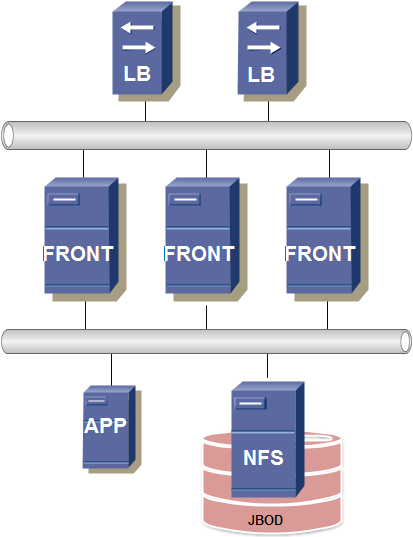
\includegraphics[width=1.0\textwidth]{IM}
    \caption{Arquitectura \label{fig:centralized}}    
\end{figure}

S'exposaran en primer lloc les capes que es trobin més a prop d'internet i s'anirà aprofundint.

En primer lloc, hi ha la capa de balanceig de càrrega o "proxy invers". Aquestes màquines rebran peticions web directament dels clients i les enrutaran cap el següent nivell. Tindran la finalitat de prendre la decissió de quina màquina rebrà la petició web. També seran terminadors SSL; actuaran de firewalls, doncs només enrutaran el tràfic per ports (de nivell 4) legítims, i seran la capa visible de la aplicació a internet.

En segon lloc, hi haurà la capa de "Frontals Web". Aquestes màquines tindran la capacitat de processar la petició web i enrutar aquelles parts que depenguin de codi dinàmic cap a la següent capa. Un cop la següent capa retorni els resultats tindran la capacitat de formatar la presentació de la resposta HTTP. D'altre banda, i com a punt més important, disposaran de gran part del contingut estàtic de l'aplicació. Donat que hi haurà volums molt grans de binaris, s'ha obtat perquè aquesta capa actuï com a cache de disc de les imatges de l'aplicació i del codi estàtic que s'executa al client. Les opciones inicials eren, o bé disposar d'un sistema d'emmagatzematge centralitzat amb totes les imatges o que tots els nodes de la capa disposesin de tots els fitxers estàtics. Donat que es va creure que ambdues eren solucions amb inconvenients insalvables per costos econòmics o per problemes de concurrència, es va optar per la solució de disposar d'alguns fitxers a cada node maximitzant aquells fitxers que més s'utilitzin.
Amb aquesta decisió s'aconsegueix minimitzar l'espai de disc de les màquines d'aquesta capa, però sense perdre rendiment en quan a latències de xarxa. Val a dir, que permetrà paral·lelitzar l'ample de banda de la xarxa a l'hora d'accedir a les imatges i no saturar la capa d'emmagatzematge. A més a més, permet que l'aplicació escali en capacitat d'usuaris de manera relativament senzilla. Evidentment fins a límits marcats per l'ample de banda de la xarxa de sortida a internet.   

A continuació, hi haurà la capa d'aplicació. Es tracte de nodes que executaran aquelles parts de codi necessaries per desenvolupar la lògica de negoci de l'aplicació. Serà una capa que no tindrà un pes molt important perquè es tracta d'una aplicació amb un ús intensiu en contingut estàtic. No obstant, val a dir que es tractaria d'una capa molt important si l'aplicació web fos d'un altre tipus.
Com a afegit d'aquesta cap hi haurà un servidor d'índexos que permeti cercar imatges eficientment. Es podria contemplar com una altre capa, però s'ha determinat que és una part poc rellevant de la plataforma. És per això que el indexador no disposarà d'alta disponibilitat.

Finalment hi ha la capa d'emmagatzematge. Constarà de dues parts, en primer lloc una solució de cabina de discs SAN que permetrà crear volums a partir dels discs existents així com afegir més discs. En segon lloc hi haurà els servidors de storage. Un clúster de nfs que serà exportat principalment als Frontals. Les dades cachejades dels Frontals seran originalment d'aquests servidors.


\section{Workloads}

Actualment el dimensionament de la plataforma no està definit perquè cal determinar una manera adequada de contabilitzar les càrregues que pot assumir la plataforma. No obstant, cada capa haurà de disposar de com a mínim dos nodes per poder garantir l'alta disponibilitat.

Un avantatge pel qual s'han desacoblat les capes en diferents nivells és per poder disposar de diferents prestacions de màquines en els diferents nivells i que cadascun disposi de nodes homogenis. Guanyant en granularitat a l'hora d'escollir components per satisfer els workloads així com minimitzar els costos.

Per això, cal determinar el tipus de càrregues que tindrà cada capa. En conseqüència es tractarà de definir les necessitats de cada node idealment.

\begin{description}

\item[Load Balancers] Únicamnet cal que siguin nodes ràpids a l'hora de fer operacions de I/O de xarxa. Per tant, seran nodes que no necesitaran gaire espai de disc, ni velocitat en aquest.

\item[Frontals] Seran nodes que tindran càrrega de IOPS en forma de sol·licituds de transferència de fitxers. Per tant, caldran màquines amb discs ràpids i espais de memòria prou grans. No obstant, seran nodes amb poca capacitat de càlcul.

\item[Servidors d'aplicacions]
Seran nodes que tindran principalment capacitat de càlcul. No els caldrà gaire espai de disc.

\item[Emmagatzematge]
Aquesta capa necesitarà molt d'espai de disc, no necessariament ràpid. Haurà de ser storage robust i disposar d'un ample de banda de xarxa important. Aquests nodes no necesitaran capacitat de càlcul.

\end{description}

Els càlculs per determinar el rendiment de la plataforma en requests/segon s'han dut a terme tenint en compte el nombre de Herzts que podrien disposar els nodes de cada capa. No obstant, s'han descartat perquè no tenen el rigor que es creu necessari per desenvolupar el projecte. 
S'ha tractat d'assingar pesos a les diferents capes de la plataforma i així determinar el nombre de nodes per capa. Aquesta solució no ha estat adequada, perquè s'està assumint que les peticions per segon d'una aplicació web vénen determinades per la capacitat de càlcul. Malgrat vàrem fer aquesta assumció, s'ha vist que és errònia. Més si es té en compte que es tracte d'una aplicació intensiva en servir fitxer estàtics.

És per això que s'està cercant la manera de contabilitzar les peticions servides per segon, en funció de les capacitats de la plataforma.

\section{Centre de col·locació}

De entre totes les opcions disponibles es considera més adient els serveis que ofereix la empresa Mordor Colocation Center. 

Les característiques de l’empresa Mordor Colocation Center són:

\begin{itemize}
\item Ubicada a Barcelona (Edifici @22)
\item Preu per allotjament de servidors a 14.000 euros/any * rack de 42U.
\item PUE de 1,15 - Es paga el consum energetic de les maquines amb un 15% adicional com a concepte de UPS i refrigeració.
\item Replicació N+1 de tots els elements HVAC i UPS.
\item Generador Diesel en cas de fallada eléctrica.
\item Dues línies d’entrada d’electricitat.
\item Dues línies de connexió de xarxa.
\item Certificació que garanteix un 99,982\% de uptime.
\end{itemize}

La sel·lecció s’ha dut a terme tenint en compte principalment el requisit d’alta disponibilitat de dades del servei del nou CPD. Mordor Colocation Center proporciona les millors garanties Uptime d’entre les opcions disponibles, tant per certificació de Uptime com per serveis replicats (especialment per la replicació de elements elèctrics i la doble entrada d’electricitat i xarxa).

\section{Emmagatzematge extern}
Sobre les opcions disponibles de backup extern s’ha triat els serveis oferts per la empresa Take the tapes and run.

Els requisits de l’aplicació Web 2.0, basada en un gestor d’imatges, són una comunicació vertical i una gran quantitat d’emmagatzematge. Donada aquesta situació, la opció proporcionada per Take the tapes and run es la única que proporciona backup a una ubicació externa sense afectar a l'ample de banda de sortida.

\section{Feines pendents}
En aquesta entrega hem determinat els requisits i l’arquitectura del nostre CPD, per determinar els següents punts hem de seleccionar els dispositius per saber els preus i costos de cada part i poder fer una estimació adecuada de cada punt.

D’altra banda, és necessari fer una llista inicial de possibles riscos que pot tenir el CPD, per tal d’obtenir la major seguretat possible. 

\end{document}



